% !TEX TS-program = PDFlatex
% !TEX encoding = UTF-8 Unicode

% Example of the Memoir class, an alternative to the default LaTeX classes such as article and book, with many added features built into the class itself.

%\documentclass[12pt,a4paper]{memoir} % for a long document
%\documentclass[french,12pt,a4paper,article]{memoir} % for a short document
\documentclass[english,12pt,article]{article} % for a short document
%\documentclass[french,12pt,a4paper]{article} % for a short document

\usepackage{babel}
\usepackage[utf8]{inputenc} % set input encoding to utf8
\usepackage{amsmath, amsthm, amssymb}
\usepackage[T1]{fontenc}   % so _, <, and > print correctly in text.
\usepackage[strings]{underscore}    % to use "_" in text

\input{amssym.def}
\input{amssym.tex}

% Don't forget to read the Memoir manual: memman.PDF
\usepackage{color}
\usepackage{pgfplotstable}
\usepackage{pgfplots}
\usetikzlibrary{plotmarks}
\usepackage[colorlinks=true,linkcolor=blue]{hyperref} 
\usepackage{graphicx}
%%% Examples of Memoir customization
%%% enable, disable or adjust these as desired

%%% PAGE DIMENSIONS
% Set up the paper to be as close as possible to both A4 & letter:
%\settrimmedsize{11in}{210mm}{*} % letter = 11in tall; a4 = 210mm wide
%\setlength{\trimtop}{0pt}
%\setlength{\trimedge}{\stockwidth}
%\addtolength{\trimedge}{-\paperwidth}
%\settypeblocksize{*}{\lxvchars}{1.618} % we want to the text block to have golden proportionals
%\setulmargins{50pt}{*}{*} % 50pt upper margins
%\setlrmargins{*}{*}{1.618} % golden ratio again for left/right margins
%\setheaderspaces{*}{*}{1.618}
%\checkandfixthelayout 
% This is from memman.PDF

\newcommand{\latex}{\LaTeX\xspace}
\newcommand{\tex}{\TeX\xspace}
 
\def\th#1{theorem~\ref{#1}}
\def\Th#1{Theorem~\ref{#1}}
\def\eq#1{\rm Eq.~(\ref{#1})}
\def\Eq#1{\rm Eq.~(\ref{#1})}
\def\eqs#1{\rm Eqs.~(\ref{#1})}
\def\eqe#1{(\ref{#1})}
\def\sec#1{\rm Sec.~(\ref{#1})}
\def\secs#1{\rm Secs.~(\ref{#1})}
\def\sece#1{(\ref{#1})}
\def\Fig#1{\rm Figure {\rm \ref{#1}}}
\def\fig#1{\rm Figure {\rm \ref{#1}}}
\def\fige#1{ {\rm \ref{#1}}}
\def\figs#1{\rm Figures {\rm \ref{#1}}}

\definecolor{darkgreen}{rgb}{0,0.8,0.2}
\definecolor{mauve}{rgb}{0.88,0.69,1.0}
\definecolor{morve}{rgb}{0.58,0.7,0.39}
\definecolor{darkred}{rgb}{0.58,0.0,0.0}
%\definecolor{ered}{rgb}{1.0,0.0,0.0}
\definecolor{ered}{rgb}{0.0,0.0,0.0}   % ered devient noir
\definecolor{pion}{rgb}{0.01.0,1.0}
%\frenchspacing
\usepackage{pdfpages}
 

\title{ \protect \large Manual for FPP:   The Fully Polymorphic Package}    
\newcommand{\subtitle}{Using examples from  PTC and BMAD }
\author{Étienne Forest \\ Tsukuba, Japon }
%\date{12 avril 2018} 
%\date{21 juillet 2018} % Delete this line to display the current date

\bibliographystyle{prsty}
  
\begin{document}
 
\maketitle

\newpage 
{\footnotesize
\tableofcontents % the asterisk means that the contents itself isn't put into the ToC
}
\newpage 

%--------------------------------------------------------------
\section{Introduction to FPP/PTC}
\label{sec:fppptc}

\begin{figure}[tb]
  \centering
  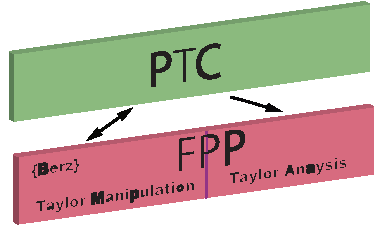
\includegraphics{FPP-PTC.pdf}
  \caption{The Fully Polymorphic Package (FPP) part of the FPP/PTC library provides manipulation and analysis of Taylor series and maps and the Polymorphic Tracking Code (PTC) part provides the physics from which accelerators can be analyzed.}
  \label{f:fpp-ptc}
\end{figure}

%--------------------------------------------------------------
\subsection{FPP and PTC}

FPP/PTC is an object oriented, open source, subroutine library for
\begin{enumerate}
\item The manipulation and analysis of Taylor series and Taylor maps.
\item Modeling of charged particle beams in accelerators using Taylor maps.
\end{enumerate}

FPP/PTC has two parts. The Fully Polymorphic Package (FPP) is the part that deals with Taylor series and maps. FPP is pure math independent of any "physics". The Polymorphic Tracking Code (PTC) part of the library deals with the modeling of particle beams and accelerators. PTC contains the "physics" and relies on FPP for manipulating Taylor maps. This is illustrated in \Fig{f:fpp-ptc}. Roughly, FPP can be subdivided into two parts, a Taylor manipulation part for basic manipulations of Taylor series and an analysis part to do things like normal form analysis. PTC uses the Taylor manipulation part of FPP for things like the construction of Taylor maps. Additionally, PTC uses the analysis tools of FPP. A closer look at FPP shows the existence of a Differential Algebra (DA) package within FPP. This package was originally coded by Martin Berz.

%--------------------------------------------------------------
\subsection{Where to Obtain FPP/PTC}

%--------------------------------------------------------------
\subsection{Concepts}

FPP/PTC is written in object oriented Fortran2008. 

FPP/PTC uses double precision real numbers defined using the type "real(dp)" "dp" is defined in FPP/PTC to correspond to double precision. For example, to define in a program a real number named "time" one would write:
\begin{verbatim}
  real(rp) time
\end{verbatim}

In Fortran, a "structure" (also called a "derived type") is like a struct in C or a class in C++. That is, a structure holds a set of components as defined by the programmer. With FPP, the "taylor" structure is used to hold a taylor series. The definition of the taylor type, as given in the file h_definition.f90 in the FPP/PTC library, is
{\footnotesize
\begin{verbatim}
  TYPE TAYLOR
     INTEGER I       !  integer I is a pointer in old da-package of Berz
  END TYPE TAYLOR
\end{verbatim}
}
The details of how a Taylor series is stored in the structure is not important here. What is important is that this structure can be used to hold a taylor series.

For practical calculations it is often not convenient to deal directly with the taylor structure. For reasons that will be discussed later, the preferred structure to use is a polymorphic structure called "real_8". In general, a "polymorphic" variable is a variable that can act in different ways depending on the context of the program. Here, a real_8 variable can act as if it where a real number or it can act as if it were a Taylor series depending upon how it is initialized.
An example program will make this clear.

{\footnotesize
\begin{verbatim}
  program real_8_example
  use pointer_lattice   ! Read in structure definitions, etc.
  implicit none

  type (real_8) r8      ! Define a real_8 variable named r8
  real(dp) x            ! Define a double precision number

  !

  long_print = .false.        ! Shorten "call print" output
  call init (only_2d0, 3, 0)  ! Initialize FPP/PTC. #Variables = 2, Order = 3

  x = 0.1d0
  call alloc(r8)          ! Initialize memory for r8
  r8 = x                  ! This will make r8 act as a real

  print *, 'Print r8 acting as a real:'
  call print (r8)

  r8 = 0.7d0 + dz_8(1) + 2*dz_8(2)**3 ! This will make r8 act as a Taylor series
  print *, 'Print r8 acting as a Taylor series:'
  call print(r8)

  r8 = r8**4  ! Raise the Taylor series to the 4th power
  print *, 'Series (0.7d0 + z1)**4:'
  call print (r8)

  call kill(r8)
  end program
\end{verbatim}
}

The lines
\begin{verbatim}
  call print (r8)
\end{verbatim}
print the "value" of r8. When r8 is acting as a real number, as in the first call print statement, the output is just a real number:
{\scriptsize
\begin{verbatim}
  Print r8 acting as a Taylor series:
  0.100000000000000
\end{verbatim}
}

When r8 is acting as a Taylor series the call print statement prints out the Taylor series. Thus the output of the second call print is:
{\scriptsize
\begin{verbatim}
  Print r8 acting as a Taylor series:
Properties, NO =    3, NV =    2, INA =   21
 *********************************************

   0  0.7000000000000000       0  0
   1   1.000000000000000       1  0
\end{verbatim}
}
Some explanation is required here. The initialization of FPP/PTC was done by the line
{\scriptsize
\begin{verbatim}
  call init (only_2d0, 3, 0)  ! Initialize FPP/PTC. #Variables = 2, Order = 3
\end{verbatim}
}
This setup FPP/PTC to 


\begin{verbatim}
  long_print = .false.
\end{verbatim}
makes the output of 



  TYPE REAL_8
     TYPE (TAYLOR) T      !  USED IF TAYLOR
     REAL(DP) R           !    USED IF REAL
     INTEGER KIND  !  0,1,2,3 (1=REAL,2=TAYLOR,3=TAYLOR KNOB, 0=SPECIAL)
     INTEGER I   !   USED FOR KNOBS AND SPECIAL KIND=0
     REAL(DP) S   !   SCALING FOR KNOBS AND SPECIAL KIND=0
     LOGICAL(LP) :: ALLOC  1 IF TAYLOR IS ALLOCATED IN DA-PACKAGE
  END TYPE REAL_8



\bibliography{nlinear}


\end{document}



